\clearpage
\section{Theoretical motivation\label{sec:theory}}

\subsection{The Standard Model\label{sec:SM}}

Particle physics concerns itself with the study of particles and fields. 
Our current knowledge of their characteristics and interactions are formalized
in the quantum field theory called the Standard Model~\cite{bettini2014introduction,griffiths2008introduction}
which relies upon symmetry 
principles. The global symmetry group of the Standard Model is given by three symmetries: 
the color charge symmetry of Quantum Chromo Dynamics (QCD) represented in SU(3), 
the flavor symmetry of Quantum Flavor Dynamics (QFD) represented in SU(2) and the electric charge symmetry of Quantum 
Electro Dynamics represented in U(1). Together, SU(3) $\times$  SU(2) $\times$ U(1) requires 
the SM Lagrangian be invariant under local gauge transformations~\cite{perkins2000introduction}. It describes the electron ($e$), 
muon ($\mu$), and tau ($\tau$) leptons, all with spin 1/2 and electric charge -1, and their 
associated neutral, massless, spin-1/2 neutrinos $\nu_{e}$, $\nu_{\mu}$, $\nu_{\tau}$. 
They are arranged into SU(2) doublets of weak isospin $(\nu_{l}, l)_L$ of left-handed
states, and singlets $l_R$ of right-handed states. Extending the SM to include massive
neutrinos, as required by the observation of neutrino flavor oscillations, is discussed
in Ref.~\cite{griffiths2008introduction}.
The spin-1/2 quarks are similarly arranged into three ``generations'': $(u, d), (c, s),
(t, b)$, with electric charges (+2/3, −1/3). They carry color charge, and their weak
interactions take place among a set of states mixed by a rotation matrix. Quarks
are not observed free, but rather as the elementary constituents of color-
neutral composite hadrons.
The interactions among particles are mediated by spin-1 bosons: eight electrically
neutral, massless gluons (carrying color charges) mediate strong interactions; the neutral, 
massless photon $\gamma$ mediates electromagnetism; and the massive $W^\pm$ and $Z^0$ mediate 
the weak interactions. Spontaneous breaking  of the electroweak SU(2) $\times$ U(1)
symmetry gives masses to the $W$ and $Z$, and further gives rise to the neutral, spin-
0 Higgs particle $H^0$, with a positive vacuum expectation value. The SM contains
19 parameters~\cite{perkins2000introduction}, usually taken to be the three lepton masses, six quark masses,
four parameters characterizing generational mixing among the quarks, three coupling
strengths, the masses of the $Z$ and $H$, and a coefficient allowing for the violation of
combined charge-conjugation and parity-inversion symmetry in strong interactions.
(The description of neutrino mass requires additional parameters.)
The success of the SM at predicting and interpreting experimental results is
tremendous: all of the leptons, quarks, and gauge bosons have been observed, and
interact according to the SM at length scales down to approximately $10^{-18}$~m~\cite{perkins2000introduction}.
Despite its broad success, however, the SM remains incomplete: the nature of neutrino
masses and their mixing is not yet determined; it is not known how to incorporate
the observed dark matter (should it consist of particles), nor the effects of gravity,
which are expected to become relevant at high energies. In addition, the mass of the
scalar Higgs, $m_H$, is not predicted, and ${m_{H}}^2$ receives contributions
via virtual particle loops that depend quadratically on the momentum cut-off used,
i.e. the scale at which new physics shall enter the calculation. Assuming that $m_H$ is
$\mathcal{O}$(100)~\GeV, as is required for $WW$ scattering to remain perturbative, then either
(a) new physics enters at the scale of $\mathcal{O}$(1 TeV), or (b) some mechanism is required
to remove this quadratic divergence, $e.g.$ supersymmetry~\cite{Martin:1997ns}.
\subsection{Supersymmetry\label{sec:SUSY}}

Supersymmetry is a theory of new physics that posits a new symmetry between
bosons and fermions as an extension to the standard model. SUSY is appealing for several
reasons. It allows for cancellation of quadratic divergences that appear in higher-order
corrections to the calculation of the Higgs boson mass, because terms of opposite sign
are contributed by the bosonic and fermionic superpartners. The
lightest supersymmetric particle (LSP) in R-parity conserving models, described below, is usually neutral,
massive, and weakly interacting, SUSY thus provides a candidate for dark matter. Finally,
SUSY provides a mechanism whereby the coupling constants from the three standard model
symmetry groups can be unified at a high scale, leading to the possibility of an even more
fundamental theory, i.e., a “grand unified theory” (GUT)~\cite{wess1992supersymmetry}.\\
\indent The theoretical underpinnings of SUSY rely upon a symmetry that relates bosons
to fermions. In SUSY, the fundamental particle content of the universe will at least double,
as all standard model particles will have a SUSY partner. 
%For a minimal extension of the
%standard model, the particle content, along with the relationship to standard matter, %is
%shown in Table 2.1. 
The scalar superpartners of the fermions are called sfermions and have a spin 0. The fermionic 
superpartners of the bosons are called bosinos and half-integer spins. The names of the individual
particles can be constructed in a similar manner.
SUSY can be realized in many ways and it is important to choose a model that is
consistent and yet feasible to study. A completely unconstrained minimal parametrization
of SUSY contains over 100 free parameters. It is necessary to reduce the number of free
parameters in order to effectively test the predictions of the theory, so certain assumptions
are made to construct a consistent model with fewer free parameters. As superpartners
have not yet been observed, their masses must be higher than the corresponding standard
model particles. This necessarily means that SUSY is a broken symmetry, and the unknown
mechanism providing the SUSY breaking can determine the type of physics one can expect
to observe. Some commonly studied models, such as mSUGRA (minimal SUper GRAvity)
and the cMSSM (constrained Minimal Supersymmetric Standard Model), posit that gravity
is responsible for providing the SUSY breaking.

\subsection{R-parity and a candidate for dark matter}

R-parity, sometimes known as matter parity, is an additional symmetry (similar to
the parity symmetry of the standard model) that determines the possible decays available
in SUSY models. R-parity is defined in Equation~\ref{eq:r-par}, where B is the baryon number, L is the
lepton number, and s is the spin of the particle in question. R-parity is a multiplicative
quantum number, with R = 1 for ordinary standard model particles and R = -1 for SUSY sparticles.

\begin{equation}
\label{eq:r-par}
R = \left(-1\right)^{3B+L+2s}
\end{equation}

R-parity-conserving models are preferred due to consequences of R-parity violating (RPV)
models, which allow for the decay of the proton, among other currently unobserved decays. 
While RPV models are not excluded, current theoretical prejudice favors R-parity 
conserving models.
If R-parity is conserved, this necessarily implies that a sparticle must be produced
in conjunction with another sparticle, i.e., sparticles will always pair produced at collider
experiments. Another consequence is that the LSP must be stable. Additionally, if the LSP
is neutral, it will be noninteracting and thus a good candidate for cold dark matter. The
neutral LSP is preferred in many models being explored at the LHC due to cosmological
constraints on exotic matter~\cite{wess1992supersymmetry}.

\subsection{Experimental signature}
\label{sec:signature}

Color confinement in QCD prohibits the isolation of quarks~\cite{Ellis:1991qj} 
and as such, when a high energy quark is produced, e.g. 
from a collision of other particles, it quickly fragments into a 
color-neutral hadron. If the quarks in the hadron have enough energy, 
they fragment again into other hadrons. This hadronization process 
continues until the resulting particles are of low enough energy that it
is no longer energetically favorable to fragment. The hadronic shower of
 particles can be clustered into objects called ``jets''. A simulation 
of such a jet is shown in Figure~\ref{fig:jets}.  

\begin{figure}[h!t]
  \begin{center}
       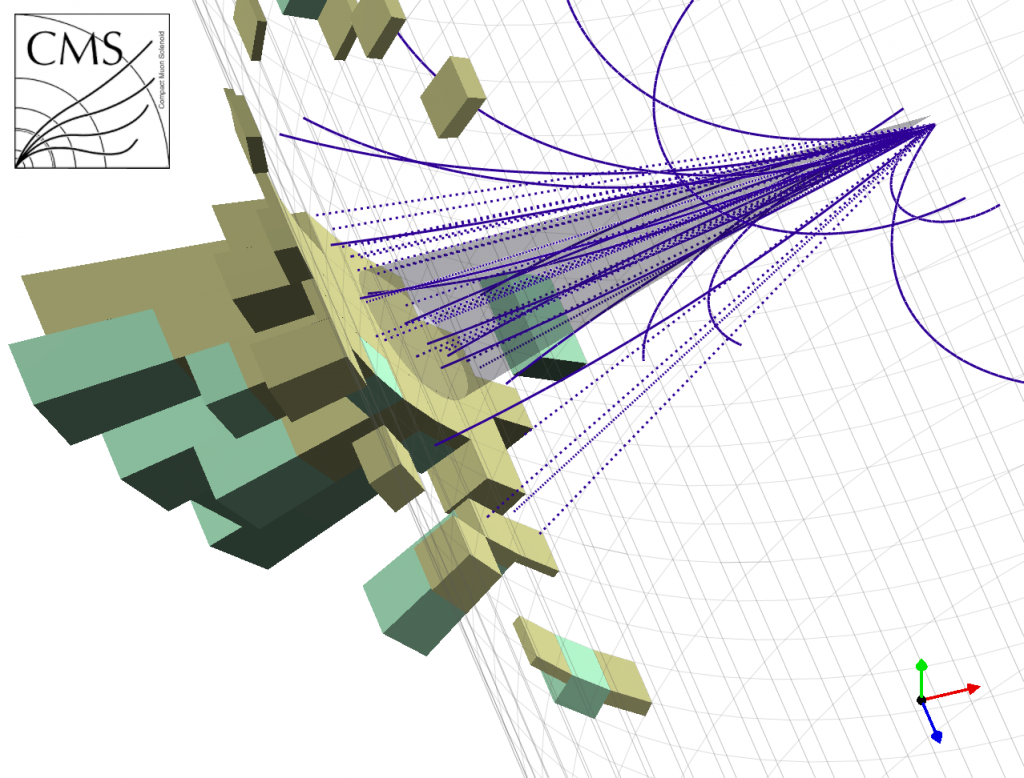
\includegraphics[width=0.45\textwidth,]{figures/JetConeAndPFJet.png}
       \caption{A simulation of a hadronized quark in the CMS detector. The
       resulting particles from hadronization are grouped into a jet (gray cone). }
    \label{fig:jets}
  \end{center}
\end{figure}

In this analysis, a search for excess in events consisting of jets and 
missing energy is conducted. This final state is expected when pairs of
heavy squarks or gluinos are produced and decay hadronically to SM quarks,
gluons, and neutralino, which escape the detector leaving only a signature
of missing energy.
%Such an excess would not directly validate a 
%supersymmetric extension of the Standard Model, since other interpretation are 
%possible, but nonetheless supersymmetry provides a extensive framework for interpretation. 
The full unconstrained SUSY theory is parametrized by over 100 variables, representing 
masses, phases and mixing angles, but it can be simplified. These simplified supersymmetric 
models (SMS) are limits of more general new-physics scenarios, where all but a few 
particles are integrated out~\cite{Alves:2011wf}.
The dominant contribution to the divergence of the Higgs boson mass arises from 
loop diagrams involving the top quark; these can be largely canceled if a scalar 
partner of the top quark (top squark) exists and has a mass below 
$\sim\!\!1\TeV$~\cite{Alves:2011wf}.
This relatively low mass is a motivation to interpret the results of this 
analysis in two decay channels of the direct pair-produced top squark. 
In the first channel, where the top squark decays to a top quark (followed by a 
semi-leptonic decay: $t \ra Wb \ra l \nu b$), provides the highest reach in probing the mass
of the top squark. The second decay scenario has only been recently pursued. It puts 
the mass difference between the top squark and the neutralino at 80~\GeV or 
less, resulting in the top squark decaying directly into a charm quark. 
Figure~\ref{fig:feynman_sms} shows the schematic diagrams of these two decay channels. 
More detailed description of each model is left for Section~\ref{sec:signal}

\begin{figure}[ht!]
  \begin{center}
    \subfigure[\label{fig:feyn_t2tt}]{
      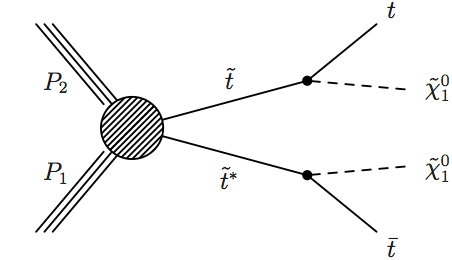
\includegraphics[width=0.45\textwidth,]{figures/T2tt}
    } 
    \subfigure[\label{fig:feyn_t2cc}]{
      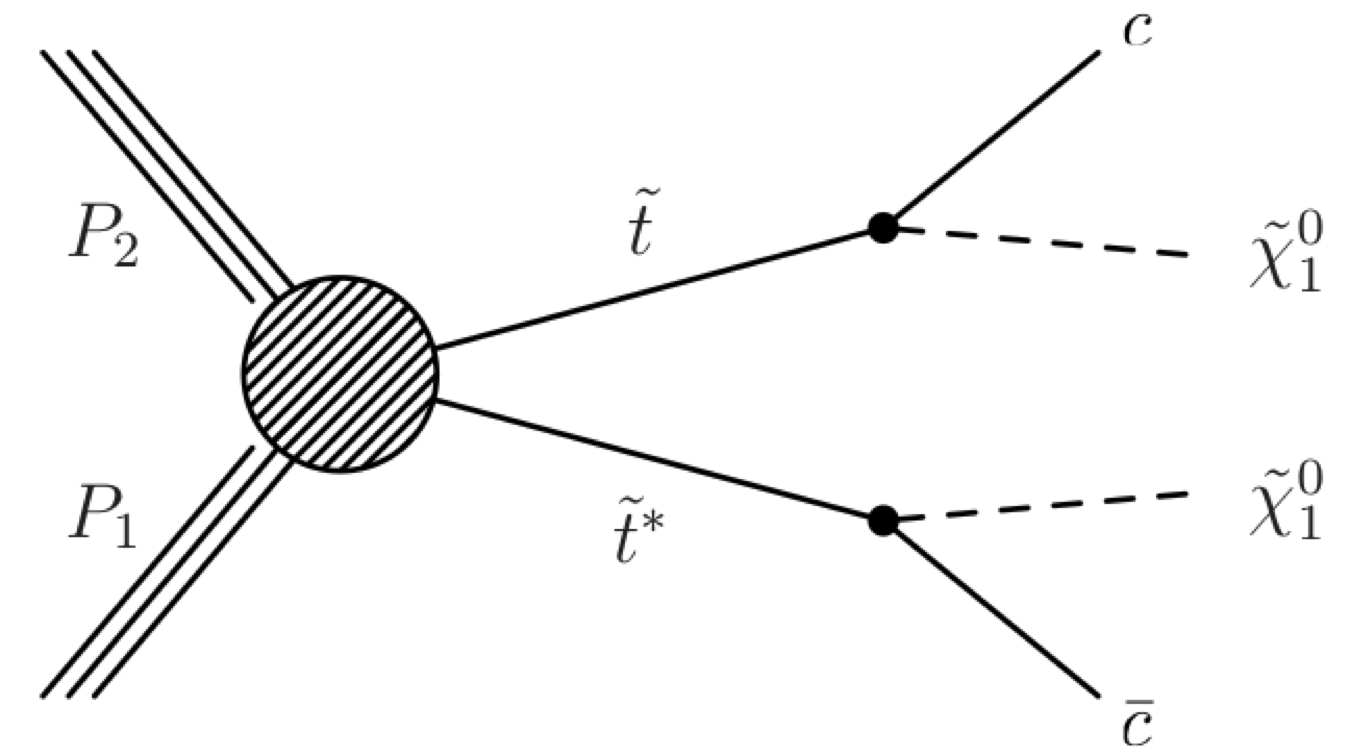
\includegraphics[width=0.45\textwidth,]{figures/T2cc}
    } \\
      \caption{Two Feynman diagrams depicting the top squark production
      and decay, in which P represents a proton, $t$ a top quark, $c$ a charm
      quark, $\st$ a top squark, \chiOnez a neutralino.}
    \label{fig:feynman_sms}
  \end{center}
\end{figure}

%\begin{figure}[ht!]
%  \begin{center}
%      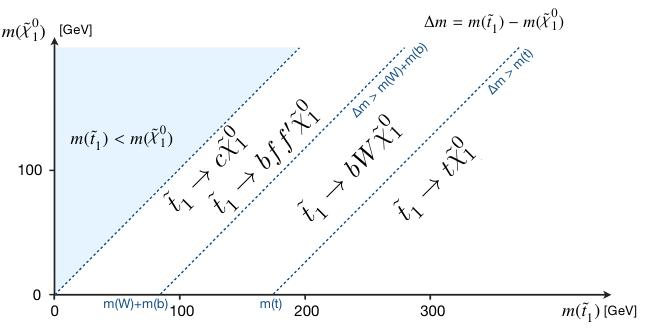
\includegraphics[width=0.45\textwidth,]{figures/mstop_mLSP_plane.jpg}
%      \caption{}
%    \label{fig:mStop_mLsp.jpg}
%  \end{center}
%\end{figure}
